\subsection*{Modelli 6 - tuning iperparametri}

L'ultimo esperimento rimasto è quello di effettuare una regolazione degli iperparametri tramite 
fine tuning. Abbiamo pertanto utilizzato lo strumento \texttt{tuner} della libreria ultralytics
per poter ricavare i valori migliori per gli iperparametri. Tale \texttt{tuner} effettua una serie 
di training con dei valori di iperparametri iniziali. Ogni iterazione consiste in una manciata
di epoche  di training necessarie per poter ottenere un modello da valutare. Alla fine di ogni 
iterazione si valuta tale modello in relazione ai suoi iperparametri. Con la nuova iterazione 
gli iperparametri vengono impostati a dei nuovi valori che vengono stabiliti dall'algoritmo del
\texttt{tuner}. L'evoluzione degli iperparametri segue un algoritmo genetico in modo da poter 
indirizzare i valori verso le prestazioni migliori.

Per far si che potessimo ottenere dei risultati consistenti anche dopo la fase di training, 
abbiamo effettuato la fase di tuning con il validation set in modo che successivamente i 
risultati non fossero influenzati da un overfitting degli iperparametri su training set.
La successiva fase di addestramento ha visto l'uso normale dei sottoinsiemi del dataset per 
train, validazione e test.

La fase di tuning è stata quella che ha richiesto più risorse, sia in termini di tempo che di 
potenza di calcolo. Nella figura \ref{fig:v6-1} è possibile vedere l'andamento della funzione 
di fitness, funzione che valutava la bontà degli iperparametri utilizzati, mentre nella figura 
\ref{fig:v6-2} l'andamento dei valori degli iperparametri nel corso del tuning.

\begin{figure}[!htb]
    \centering
    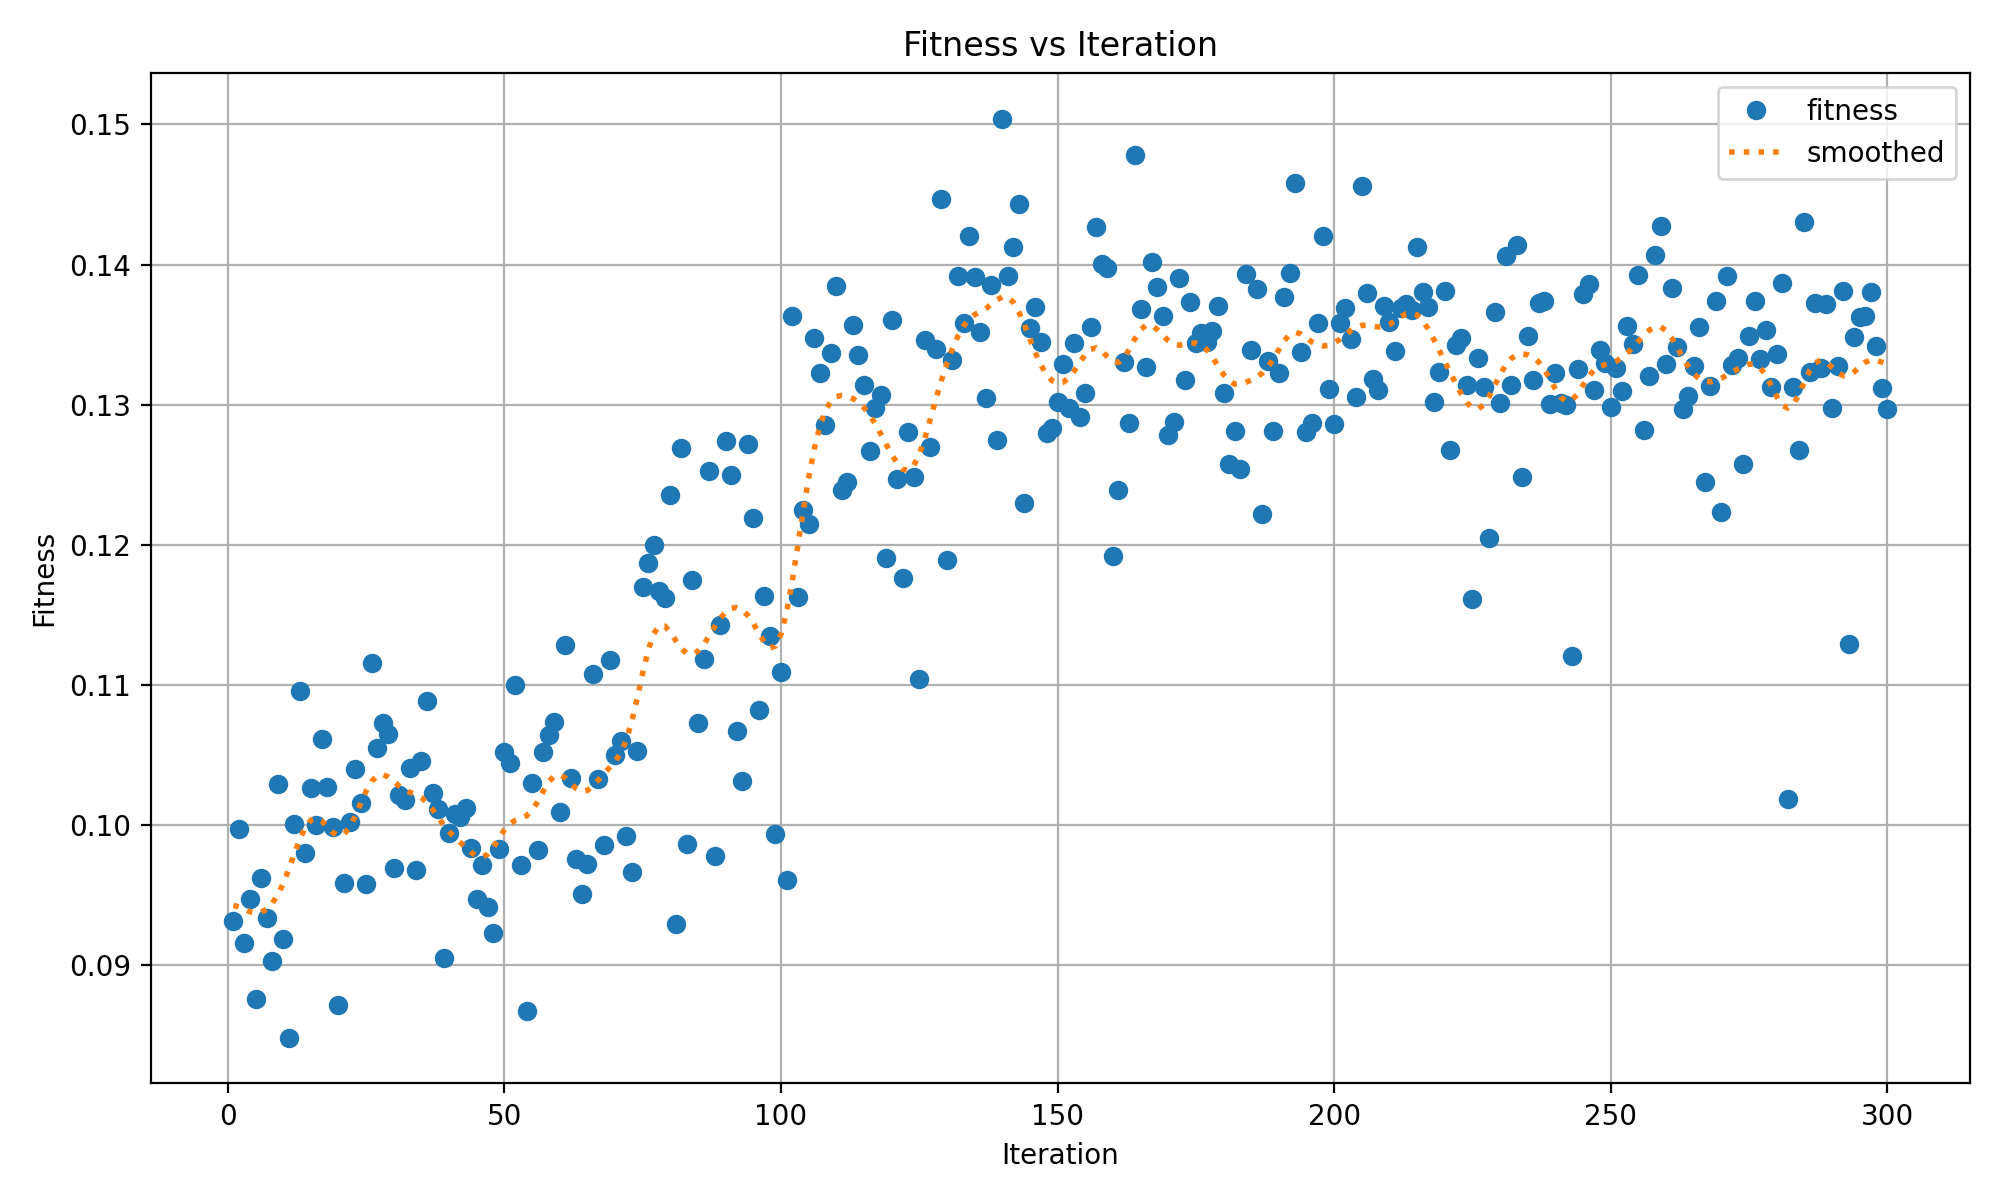
\includegraphics[width=0.8\textwidth]{v_6/tune/tune_fitness.png}
    \caption{Andamento funzioni di fitness durante l'esecuzione del tuning degli iperparametri}
    \label{fig:v6-1}
\end{figure}

\begin{figure}[!htb]
    \centering
    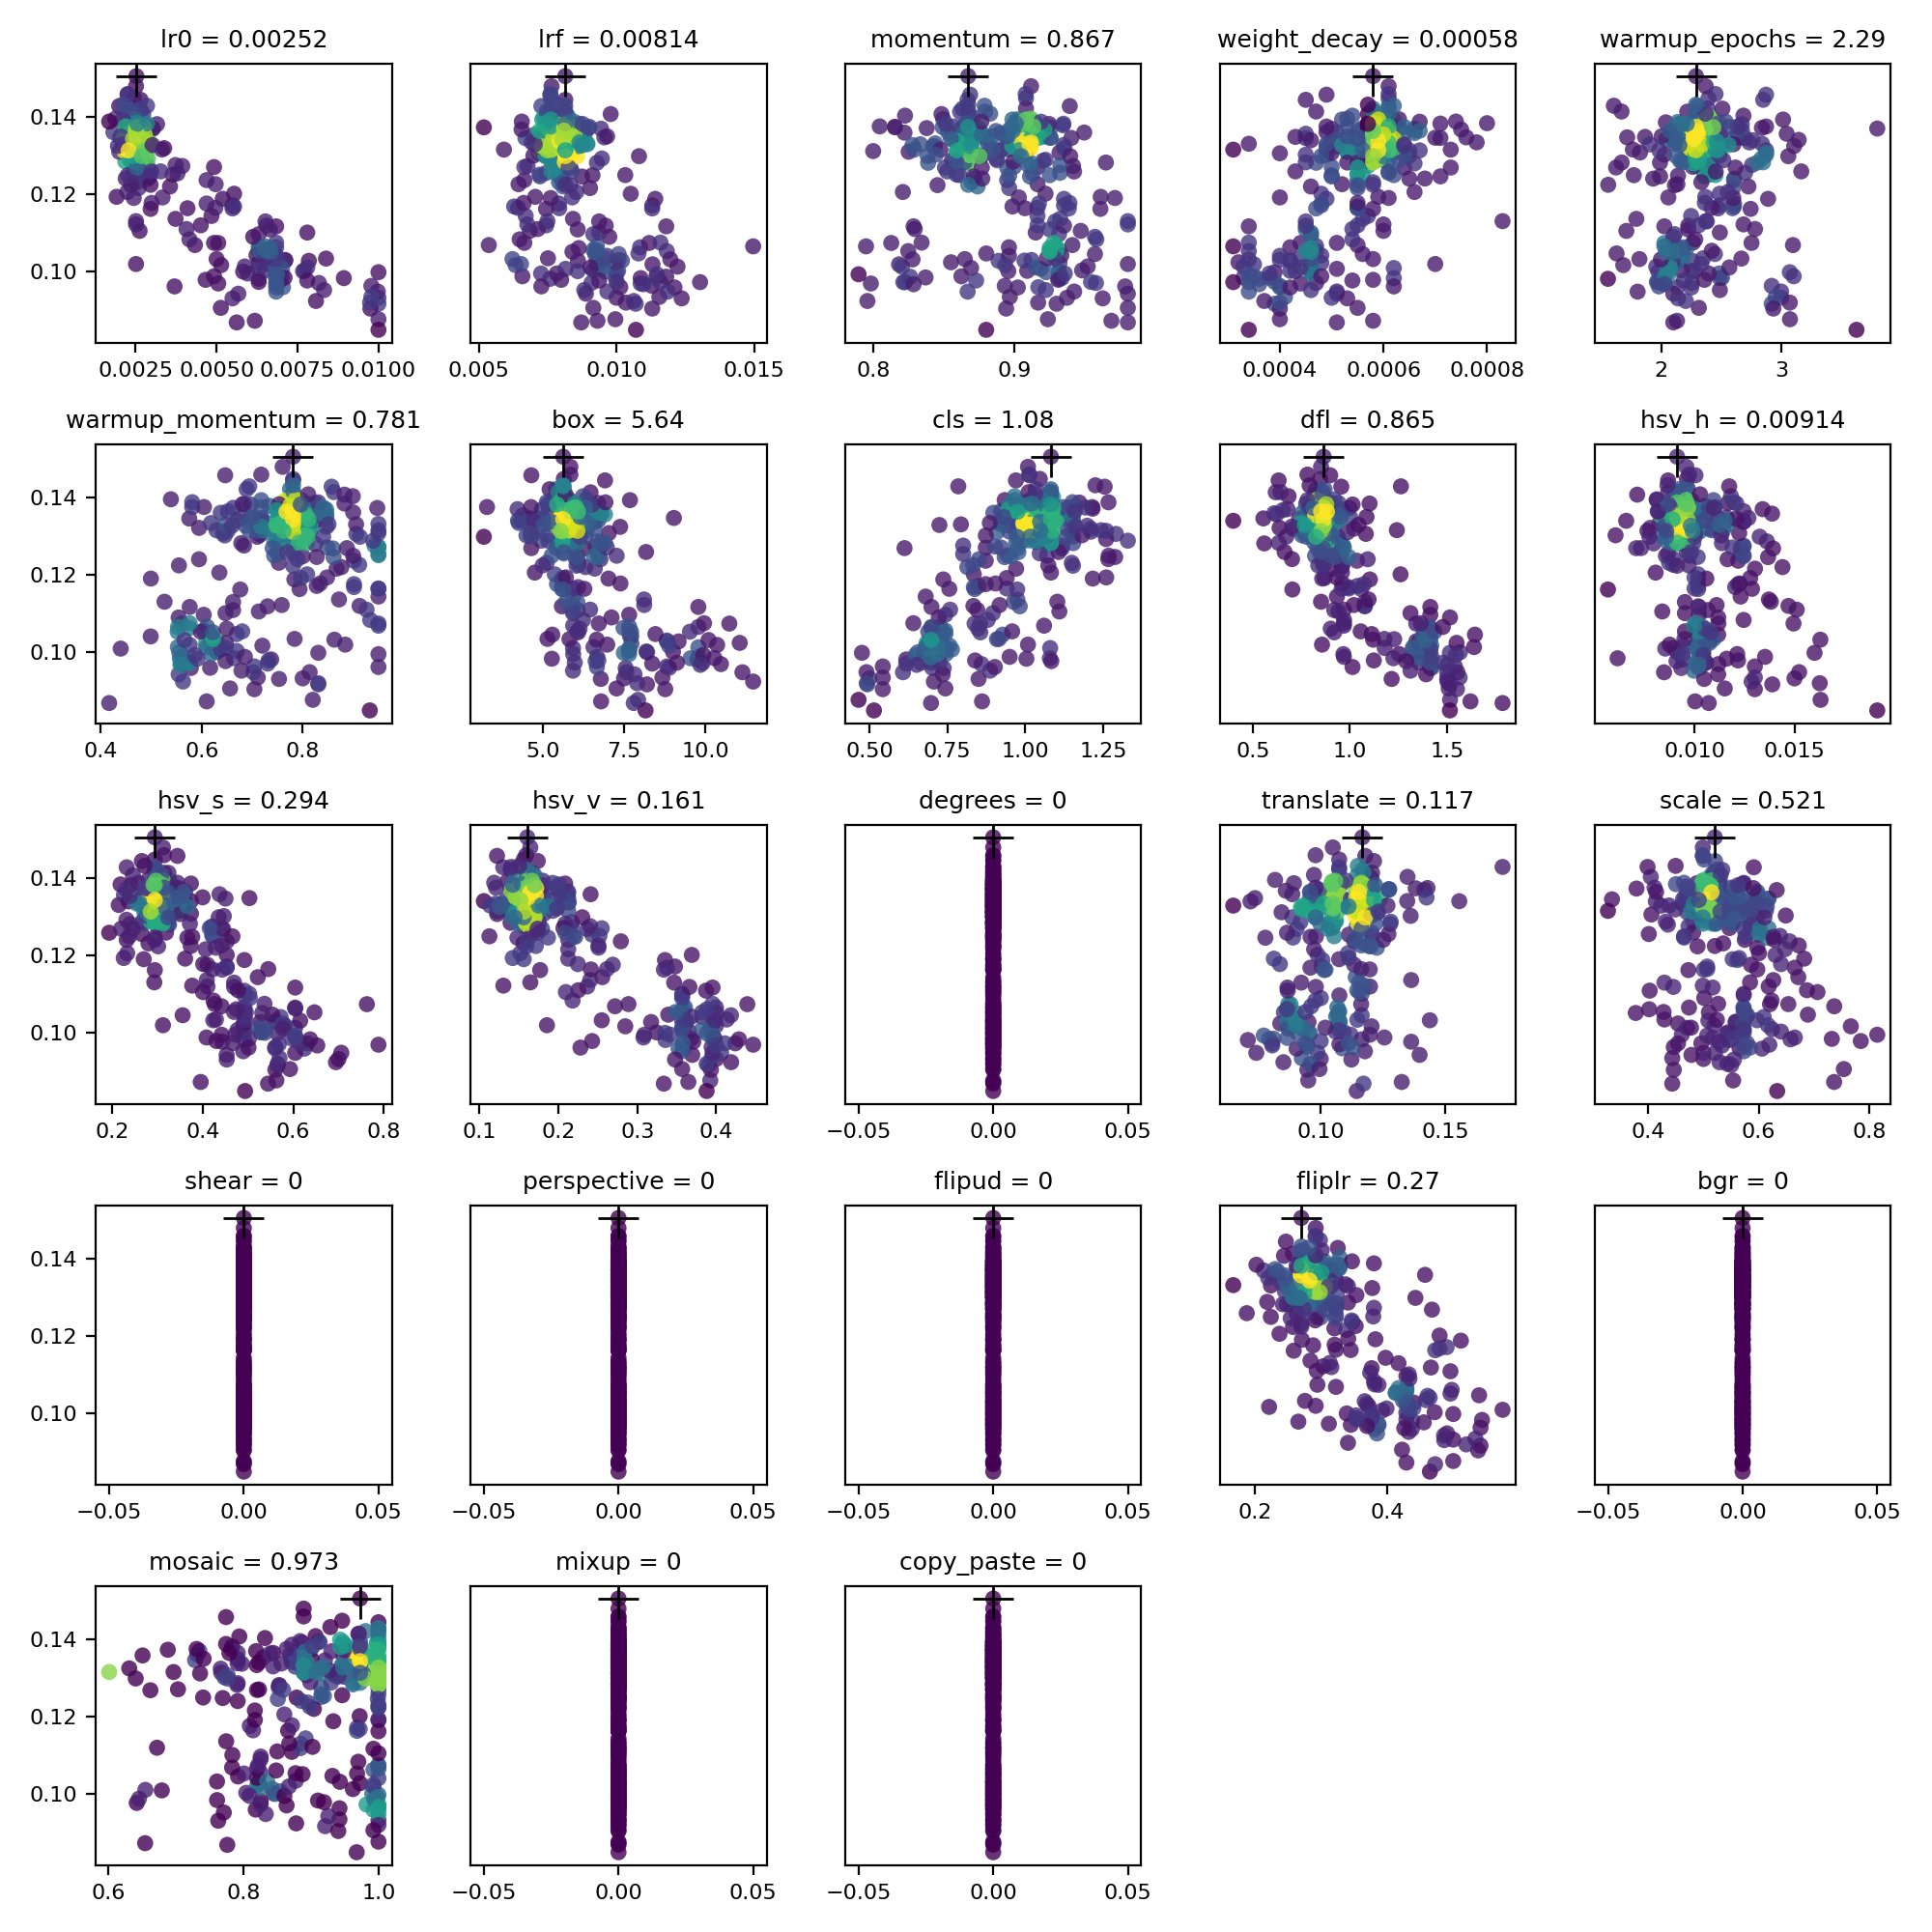
\includegraphics[width=0.8\textwidth]{v_6/tune/tune_scatter_plots.png}
    \caption{Andamento valori degli iperparametri durante la fase di tuning}
    \label{fig:v6-2}
\end{figure}

Questa fase ha visto l'utilizzo del modello nano di YOLO, YOLOv8n, per 300 iterazioni ciascuna da 
30 epoche di addestramento. Gli iperparametri migliori, poi utilizzati nella fase di training, sono 
elencati nella tabella \ref*{table:v6-1}.

\begin{table}[!htbp]
    \centering
    \begin{tabularx}{\textwidth}{lYYY}
        \toprule
        \textbf{Iperparametro} & \textbf{Valori risultati dal Tuning} & \textbf{Valore Predefinito} & \textbf{Descrizione} \\
        \midrule
        \texttt{lr0} & 0.00252 & 0.01 & Learning rate iniziale \\
        \texttt{lrf} & 0.00814 & 0.01 & Learning rate finale \\
        \texttt{momentum} & 0.86722 & 0.937 & Fattore di momentum \\
        \texttt{weight\_decay} & 0.00058 & 0.0005 & Termine di regolarizzazione per i pesi \\
        \texttt{warmup\_epochs} & 2.28985 & 3.0 & Numero di epoche di warmup \\
        \texttt{warmup\_momentum} & 0.78103 & 0.8 & Momentum iniziale durante il warmup \\
        \texttt{box} & 5.6359 & 0.05 & Guadagno della loss per il box \\
        \texttt{cls} & 1.08241 & 0.5 & Guadagno della loss per la classificazione \\
        \texttt{dfl} & 0.86478 & 1.5 & Guadagno della Distribution Focal Loss \\
        \texttt{hsv\_h} & 0.00914 & 0.015 & Fattore di aumento della tonalità \\
        \texttt{hsv\_s} & 0.29432 & 0.7 & Fattore di aumento della saturazione \\
        \texttt{hsv\_v} & 0.16061 & 0.4 & Fattore di aumento del valore \\
        \texttt{translate} & 0.11669 & 0.1 & Fattore di traslazione dell'immagine \\
        \texttt{scale} & 0.52052 & 0.5 & Fattore di scala dell'immagine \\
        \texttt{fliplr} & 0.27039 & 0.5 & Probabilità di ribaltamento orizzontale \\
        \texttt{mosaic} & 0.9728 & 1.0 & Fattore di aumento mosaic \\
        \bottomrule
    \end{tabularx}
    \caption{Risultati della sintonizzazione degli iperparametri di YOLOv8}
    \label{table:v6-1}
\end{table}

Questa configurazione è stata utilizzata per l'esecuzione di 3 addestramenti, per i modelli
\texttt{nano}, \texttt{small} e \texttt{medium} di YOLO. Ogni training ha avuto a disposizione
500 epoche con 200 epoche di \texttt{patience} prima di procedere con l'early stopping. 
\texttt{imgsz} è rimasto impostato a 800 pixel mentre come ottimizzatore è stato utilizzato AdamW.
Il nome dato ai modelli per questi training è \textit{size}\texttt{-tune-2.0}.

\begin{table}[!htb]
    \centering
    \begin{tabularx}{\textwidth}{lYYYc}
        \toprule
        Class & P & R & mAP50 & mAP50-95 \\
        \midrule
        \texttt{nano-tune-2.0} \\
        \midrule
        ALL & 0.372 & 0.428 & 0.320 & 0.159 \\
        PLASTIC\_BAG & 0.223 & 0.329 & 0.158 & 0.0463 \\
        PLASTIC\_BOTTLE & 0.714 & 0.737 & 0.751 & 0.385 \\
        OTHER\_PLASTIC\_WASTE & 0.141 & 0.385 & 0.103 & 0.0319 \\
        NOT\_PLASTIC\_WASTE & 0.409 & 0.261 & 0.268 & 0.174 \\
        \midrule
        \texttt{small-tune-2.0} \\
        \midrule
        ALL & 0.400 & 0.389 & 0.345 & 0.172 \\
        PLASTIC\_BAG & 0.273 & 0.188 & 0.205 & 0.0662 \\
        PLASTIC\_BOTTLE & 0.741 & 0.724 & 0.757 & 0.395 \\
        OTHER\_PLASTIC\_WASTE & 0.152 & 0.293 & 0.0948 & 0.0297 \\
        NOT\_PLASTIC\_WASTE & 0.433 & 0.351 & 0.321 & 0.198 \\
        \midrule
        \texttt{medium-tune-2.0} \\
        \midrule
        ALL & 0.363 & 0.487 & 0.335 & 0.166 \\
        PLASTIC\_BAG & 0.254 & 0.372 & 0.194 & 0.0628 \\
        PLASTIC\_BOTTLE & 0.737 & 0.768 & 0.769 & 0.397 \\
        OTHER\_PLASTIC\_WASTE & 0.111 & 0.475 & 0.0952 & 0.0303 \\
        NOT\_PLASTIC\_WASTE & 0.350 & 0.334 & 0.280 & 0.173 \\
        \bottomrule
    \end{tabularx}
    \caption{Risultati delle metriche sul test set per \textit{size}\texttt{-tune-2.0}}
    \label{table:v6-2}
\end{table}